\documentclass[hints,nooutcomes,noauthor,handout]{ximera}

\graphicspath{  
{./}
{./whoAreYou/}
{./drawingWithTheTurtle/}
{./bisectionMethod/}
{./circles/}
{./anglesAndRightTriangles/}
{./lawOfSines/}
{./lawOfCosines/}
{./plotter/}
{./staircases/}
{./pitch/}
{./qualityControl/}
{./symmetry/}
{./nGonBlock/}
}


%% page layout
\usepackage[cm,headings]{fullpage}
\raggedright
\setlength\headheight{13.6pt}


%% fonts
\usepackage{euler}

\usepackage{FiraMono}
\renewcommand\familydefault{\ttdefault} 
\usepackage[defaultmathsizes]{mathastext}
\usepackage[htt]{hyphenat}

\usepackage[T1]{fontenc}
\usepackage[scaled=1]{FiraSans}

%\usepackage{wedn}
\usepackage{pbsi} %% Answer font


\usepackage{cancel} %% strike through in pitch/pitch.tex


%% \usepackage{ulem} %% 
%% \renewcommand{\ULthickness}{2pt}% changes underline thickness

\tikzset{>=stealth}

\usepackage{adjustbox}

\setcounter{titlenumber}{-1}

%% journal style
\makeatletter
\newcommand\journalstyle{%
  \def\activitystyle{activity-chapter}
  \def\maketitle{%
    \addtocounter{titlenumber}{1}%
                {\flushleft\small\sffamily\bfseries\@pretitle\par\vspace{-1.5em}}%
                {\flushleft\LARGE\sffamily\bfseries\thetitlenumber\hspace{1em}\@title \par }%
                {\vskip .6em\noindent\textit\theabstract\setcounter{question}{0}\setcounter{sectiontitlenumber}{0}}%
                    \par\vspace{2em}
                    \phantomsection\addcontentsline{toc}{section}{\thetitlenumber\hspace{1em}\textbf{\@title}}%
                     }}
\makeatother



%% thm like environments
\let\question\relax
\let\endquestion\relax

\newtheoremstyle{QuestionStyle}{\topsep}{\topsep}%%% space between body and thm
		{}                      %%% Thm body font
		{}                              %%% Indent amount (empty = no indent)
		{\bfseries}            %%% Thm head font
		{)}                              %%% Punctuation after thm head
		{ }                           %%% Space after thm head
		{\thmnumber{#2}\thmnote{ \bfseries(#3)}}%%% Thm head spec
\theoremstyle{QuestionStyle}
\newtheorem{question}{}



\let\freeResponse\relax
\let\endfreeResponse\relax

%% \newtheoremstyle{ResponseStyle}{\topsep}{\topsep}%%% space between body and thm
%% 		{\wedn\bfseries}                      %%% Thm body font
%% 		{}                              %%% Indent amount (empty = no indent)
%% 		{\wedn\bfseries}            %%% Thm head font
%% 		{}                              %%% Punctuation after thm head
%% 		{3ex}                           %%% Space after thm head
%% 		{\underline{\underline{\thmname{#1}}}}%%% Thm head spec
%% \theoremstyle{ResponseStyle}

\usepackage[tikz]{mdframed}
\mdfdefinestyle{ResponseStyle}{leftmargin=1cm,linecolor=black,roundcorner=5pt,
, font=\bsifamily,}%font=\wedn\bfseries\upshape,}


\ifhandout
\NewEnviron{freeResponse}{}
\else
%\newtheorem{freeResponse}{Response:}
\newenvironment{freeResponse}{\begin{mdframed}[style=ResponseStyle]}{\end{mdframed}}
\fi



%% attempting to automate outcomes.

%% \newwrite\outcomefile
%%   \immediate\openout\outcomefile=\jobname.oc
%% \renewcommand{\outcome}[1]{\edef\theoutcomes{\theoutcomes #1~}%
%% \immediate\write\outcomefile{\unexpanded{\outcome}{#1}}}

%% \newcommand{\outcomelist}{\begin{itemize}\theoutcomes\end{itemize}}

%% \NewEnviron{listOutcomes}{\small\sffamily
%% After answering the following questions, students should be able to:
%% \begin{itemize}
%% \BODY
%% \end{itemize}
%% }
\usepackage[tikz]{mdframed}
\mdfdefinestyle{OutcomeStyle}{leftmargin=2cm,rightmargin=2cm,linecolor=black,roundcorner=5pt,
, font=\small\sffamily,}%font=\wedn\bfseries\upshape,}
\newenvironment{listOutcomes}{\begin{mdframed}[style=OutcomeStyle]After answering the following questions, students should be able to:\begin{itemize}}{\end{itemize}\end{mdframed}}



%% my commands

\newcommand{\snap}{{\bfseries\itshape\textsf{Snap!}}}
\newcommand{\flavor}{\link[\snap]{https://snap.berkeley.edu/}}
\newcommand{\mooculus}{\textsf{\textbf{MOOC}\textnormal{\textsf{ULUS}}}}


\usepackage{tkz-euclide}
\tikzstyle geometryDiagrams=[rounded corners=.5pt,ultra thick,color=black]
\colorlet{penColor}{black} % Color of a curve in a plot



\ifhandout\newcommand{\mynewpage}{\newpage}\else\newcommand{\mynewpage}{}\fi

\title{Hips and valleys}


\author{Bart Snapp}

\begin{document}
\begin{abstract}
  We compute new slopes found in roofs.
\end{abstract}
\maketitle


\begin{listOutcomes}
\item Apply the Pythagorean theorem to solve problems.
\item Extend ideas from two-dimensions to three-dimensions.
\item Follow steps in an algorithm to solve a problem.
\item Translate classroom mathematics into real world mathematics.
\end{listOutcomes}


Imagine a house where the roof where two slopes meet. This will either
form a ``hip'' or a ``valley''.
\begin{center}
  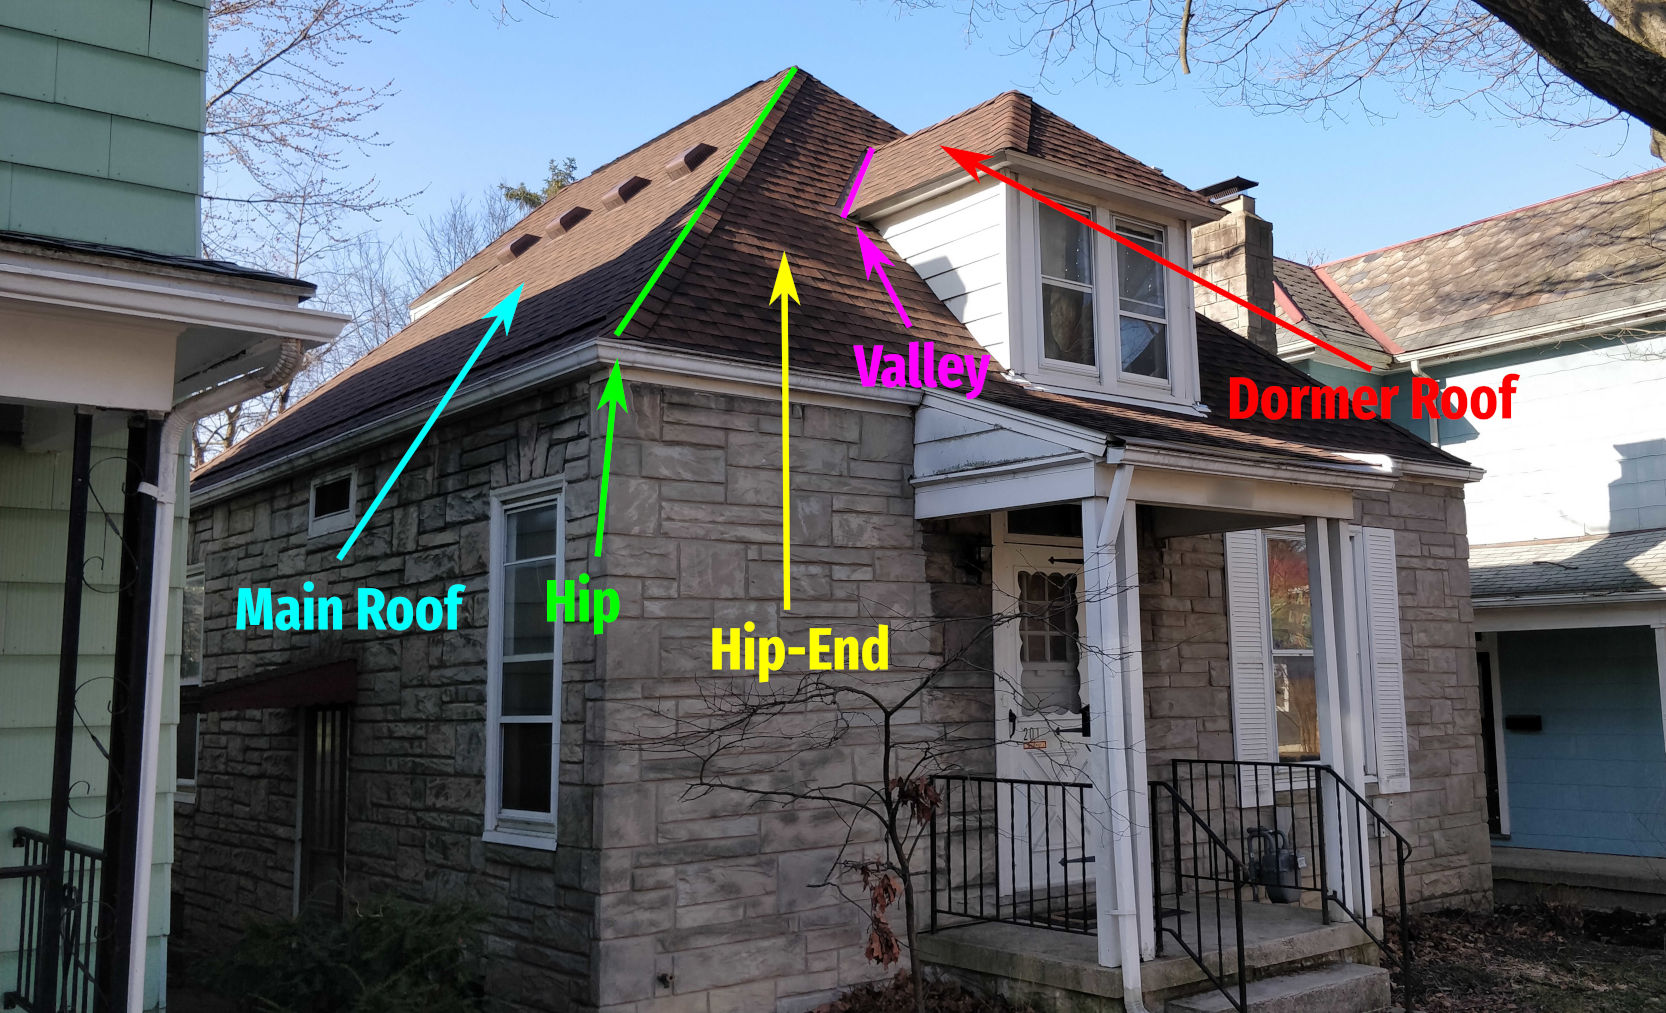
\includegraphics[width=.8\textwidth]{house.jpg}
\end{center}
Here's a question we want answered: Given the SLOPE of the roofs that
meet, What the slope (or pitch) of the hip or valley?



\mynewpage

%% \begin{question} We'll start by computing some areas.
%% \begin{enumerate}
%% \item Consider the \link[\textit{Luxor Las
%%     Vegas}]{https://en.wikipedia.org/wiki/Luxor_Las_Vegas}:
%%   \begin{center}
%%     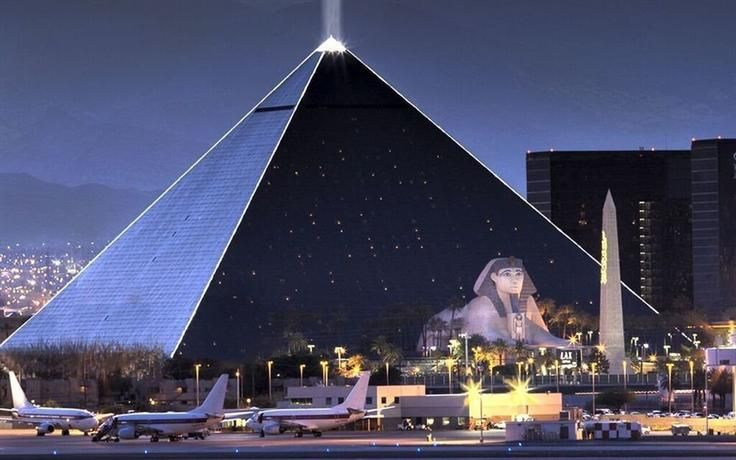
\includegraphics[width=.4\textwidth]{pyramid.jpg} 
%%   \end{center}
%%  Assuming that the (square) base of this building has a side length of
%%  $646$ feet and that the pyramid is $350$ feet tall, compute the
%% surface in square feet, not including the bottom. 
 
%% \item Here is a roof of a building that is $24\ feet$ by $12\ feet$. The slope of the hip end and the main roof are $\tfrac{6}{12}$. 
%%   \begin{center}
%%     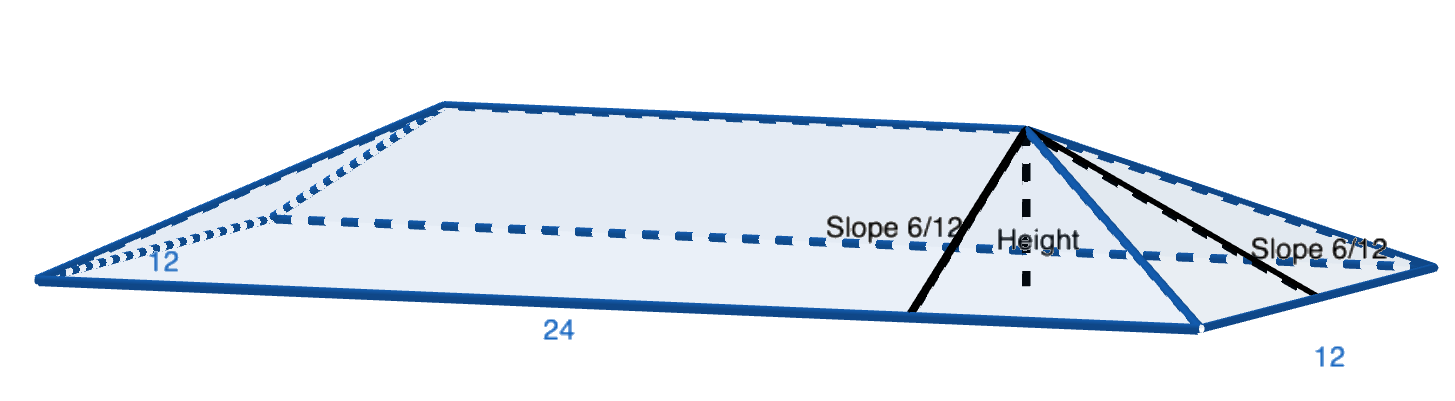
\includegraphics[width=.8\textwidth]{RoofShape} 
%%   \end{center}
  
%% Use this information to find:
%% \begin{enumerate}
%%  \item the length of the dotted line ``height,"
%%  \item the lengths of the two solid black lines,
%%  \item the length of the top of the roof,
%%  \item area of the whole roof
%% \end{enumerate}
%% A 3D model is available at \url{https://www.geogebra.org/m/zu5zsvx6}
%%  \end{enumerate}
%%  \end{question}
 
%%  \mynewpage
 
 \begin{question}
  Here are plans for a $1$-car garage that I got from \link[\textit{Garage Plans by Behm Design}]{https://behmdesign.com/shop/}:
   \begin{center}
     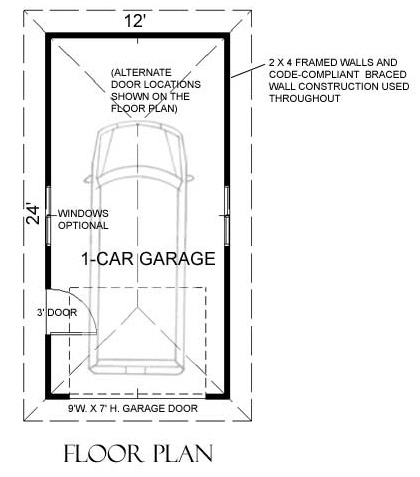
\includegraphics[width=.4\textwidth]{oneCarGarage.jpeg}
    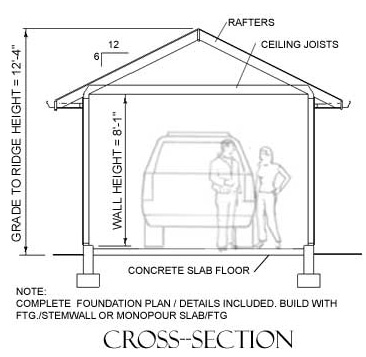
\includegraphics[width=.35\textwidth]{oneCarGarageFront.jpeg}
   \end{center}
   \begin{enumerate}
\item Assuming that the hip-end has a slope of $\tfrac{6}{12}$, and
  that the roof has an overhang of $2$ feet on all sides, find the
  area of the roof of the garage in square feet.
  %% A 3D model is available at
  %% \url{https://www.geogebra.org/m/zu5zsvx6}
  %% It seems that this might be labeled incorretly. 
 \item Considering the $1$-car garage from the previous part, now
   suppose that the hip-end has a slope of $\tfrac{8}{12}$ with an
   overhang of $2$ feet. Assume that the main roof still has a slope of $\tfrac{6}{12}$. Again find the area of the roof of the
   garage in square feet.
\end{enumerate}
In all cases above, show and explain your work.
\begin{freeResponse}
  \begin{enumerate}
    \item We must compute the height of one face of the pyramid. By
      the Pythagorean theorem, we have
      \[
      323^2 + 350^2 = h^2
      \]
      so
      \[
      h \approx 476.
      \]
      This means the top of the pyramid has a surface area of
      \[
      \text{Area} = 4\cdot \frac{646\cdot 476}{2} = 614992~\text{square feet}.
      \]
    \item Since there is an overhang of $2$ feet per side, the
      perimeter of the roof is a $16\times 28$ rectangle, meaning the
      area of the roof is AT LEAST $16\cdot 28 = 448$ square feet. If
      the main roof has a slope of $\frac{6}{12}$, it raises by
      \[
      8'\cdot \frac{6}{12}  = 4'
      \]
      This means that the height of both the main roof and the hip-end is
      \[
      \sqrt{8^2+4^2} = \sqrt{80} \approx 9~\text{feet}
      \]
      as measured along the roof. Moreover, we must move $8'$ in from
      the hip-end to achieve this height. Hence the length of the main
      ridge is
      \[
      28-8-8 = 12~\text{feet}.
      \]
      Thus the area of the roof is
      \[
      2\cdot \underbrace{\frac{16\cdot 9}{2}}_{\text{hip-end}} +
      2\left(\underbrace{2\cdot \frac{8\cdot 9}{2} + 12\cdot
        9}_{\text{main roof}}\right) = 504~\text{square feet}.
      \]
    \item Since there is an overhang of $2$ feet per side, the
      perimeter of the roof is a $16\times 28$ rectangle. If the main
      roof has a slope of $\frac{6}{12}$, it raises by
      \[
      8'\cdot \frac{6}{12}  = 4~\text{feet}
      \]
      Again, the height as measured along the main roof is
      \[
      \sqrt{8^2+4^2} = \sqrt{80}\approx 9~\text{feet}.
      \]
      Since the slope of the hip-end is $\frac{8}{12}$, and
      \begin{align*}
        x\cdot \frac{8}{12} &= 4\\
        x = \frac{12\cdot 4}{8}\\
        x = 6,
      \end{align*}
      thus must move $6'$ in from the hip-end to achieve this height.
      So the height of the hip-end (as measured along the roof) is
      \[
      \sqrt{6^2+4^2} = \sqrt{50} \approx 7~\text{feet}
      \]
      Finally, note that the length of the main ridge is
      \[
      28-6-6 = 16~\text{feet}.
      \]
      Thus the area of the roof is
      \[
      2\cdot \underbrace{\frac{16\cdot 7}{2}}_{\text{hip-end}} +
      2\left(\underbrace{2\cdot \frac{6\cdot 9}{2} + 16\cdot
        9}_{\text{main roof}}\right) = 508~\text{square feet}.
      \]
  \end{enumerate}
\end{freeResponse}


\end{question}
\mynewpage















\begin{question}
  Now let's think about the SLOPE of a hip or valley. Below we see a
  sneaky way to compute these numbers.
  \begin{mdframed}[style=OutcomeStyle]
\begin{quote}
  \textbf{Algorithm for computing the slope of a hip or valley:}

  Suppose the slopes are $\frac{s}{12}$ and $\frac{t}{12}$ with
$s\le t$.

\begin{enumerate}
\item Draw a point $O$ sitting at the intersection of a horizontal
  and vertical line.
\item Draw a vertical line segment $\bar{OS}$ where $S$ is directly
  above $O$ and $|OS| = s$.
  \item Starting from $S$, draw a line with the larger slope
    $\frac{t}{12}$ and call the intersection of this line with the
    horizontal line point $X$.
  \item Starting at point $O$, extend the line segment $\bar{OS}$ by
    drawing downward $12$ units, and call the bottom of this segment
    $B$.
     \begin{center}
        \begin{tikzpicture}[geometryDiagrams,scale=.2]
          %% \filldraw[black] (1in,1in) circle (2pt) ;
          %% \filldraw[black] (0in,0in) circle (2pt) ;
          %% \filldraw[black] (0in,1in) circle (2pt) ;
          %% \draw[<->,dashed] (1.5in,-.5in) -- (-.5in,1.5in);

          \tkzDefPoint(0,0){O}
          \tkzDefPoint(-13,0){I}
          \tkzDefPoint(1,0){nI}
          \tkzDefPoint(0,7){II}
          \tkzDefPoint(0,-13){nII}
          
          \tkzDefPoint(0,6){S}
          \tkzDefPoint(-9,0){X}
          \tkzDefPoint(-12,-2){BS}
          \tkzDefPoint(0,-12){B}

          \tkzDrawPoint[](O)
          \tkzDrawPoint[](S)
          \tkzDrawPoint[](X)
          \tkzDrawPoint[](B)
          \tkzDrawLine[ultra thin](II,nII)
          \tkzDrawLine[ultra thin](I,nI)
          \tkzDrawLine(S,BS)
          \tkzDrawSegment(O,B)
          \tkzDrawSegment[ultra thick](B,X)
          \tkzDrawSegment(O,S)

          \tkzLabelPoint(O){$O$}
          \tkzLabelPoint[](S){$S$}
          \tkzLabelPoint[above left](X){$X$}
          \tkzLabelPoint(B){$B$}

          \draw[decoration={brace,raise=.2cm,mirror},decorate,thin] (S)--(X);
          
          \node[anchor=south east] at (-5,4) {slope of $\frac{t}{12}$};
        \end{tikzpicture}
      \end{center}
  \item The slope you seek is:
    \[
    \frac{|OS|}{|BX|}\qquad \text{with a pitch of} \qquad \frac{12\cdot |OS|}{|BX|}
    \]  
\end{enumerate}
\end{quote}
  \end{mdframed}
  Let's see if we can USE the algorithm above.
  \begin{enumerate}
  \item Someone used this drawing to compute the slope of a hip.
    \begin{center}
        \begin{tikzpicture}[geometryDiagrams,scale=.2]
          %% \filldraw[black] (1in,1in) circle (2pt) ;
          %% \filldraw[black] (0in,0in) circle (2pt) ;
          %% \filldraw[black] (0in,1in) circle (2pt) ;
          %% \draw[<->,dashed] (1.5in,-.5in) -- (-.5in,1.5in);

          \tkzDefPoint(0,0){O}
          \tkzDefPoint(-13,0){I}
          \tkzDefPoint(1,0){nI}
          \tkzDefPoint(0,7){II}
          \tkzDefPoint(0,-13){nII}
          
          \tkzDefPoint(0,6){S}
          \tkzDefPoint(-9,0){X}
          \tkzDefPoint(-12,-2){BS}
          \tkzDefPoint(0,-12){B}

          \tkzDrawPoint[](O)
          \tkzDrawPoint[](S)
          \tkzDrawPoint[](X)
          \tkzDrawPoint[](B)
          \tkzDrawLine[ultra thin](II,nII)
          \tkzDrawLine[ultra thin](I,nI)
          \tkzDrawLine(S,BS)
          \tkzDrawSegment(O,B)
          \tkzDrawSegment[ultra thick](B,X)
          \tkzDrawSegment(O,S)


          \draw[decoration={brace,raise=.2cm,mirror},decorate,thin] (O)--(S);
          \node[anchor=west] at (1.5,3) {$6$};


          \draw[decoration={brace,raise=.2cm,mirror},decorate,thin] (B)--(O);
          \node[anchor=west] at (1.5,-6) {$12$};

          \draw[decoration={brace,raise=.2cm,mirror},decorate,thin] (S)--(X);
          \node[anchor=south east] at (-5,4) {slope of $\frac{8}{12}$};

          \draw[decoration={brace,raise=.2cm,mirror},decorate,thin] (X)--(B);
          \node[anchor=north east] at (-5,-6.5) {$15$};
        \end{tikzpicture}
    \end{center}
    Assuming that the slope of the main roof is larger than the slope
    of the hip-end, find the slopes (as a fraction over $12$) of the main roof, the hip-end, and
    the hip. 
  \item Suppose you have a main-roof with a slope of $\frac{4}{12}$
    and a hip-end with a slope of $\frac{7}{12}$. Either draw a
    careful picture or use
    \link[\textit{GeoGebra}]{https://www.geogebra.org/classic} to
    \textbf{find the slope of the hip.}  Show all work, explain your
    reasoning, and check your work with an \link[online
      calculator]{https://www2.strongtie.com/webapps/SlopeSkew/?source=app}.

  \end{enumerate}
  \begin{freeResponse}
    \begin{enumerate}
    \item The slope of the main roof is $\frac{6}{12}$. The slope of
      the hip-end is $\frac{8}{12}$. The slope of the hip is
      \[
      \frac{6}{15} \approx \frac{4.8}{12}.
      \]
    \item Using \textit{GeoGebra} we find:
      \begin{center}
        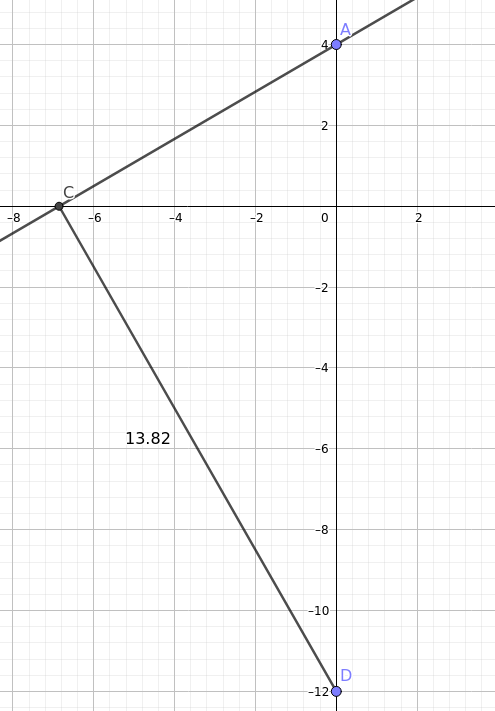
\includegraphics[width=.3\textwidth]{workUnEqSlope.png}
      \end{center}
      Hence the slope is
      \[
      \frac{4}{13.82} \approx \frac{3.5}{12}.
      \]
    \item If both slopes are the same, then our picture looks like
      this:
      \begin{center}
        \begin{tikzpicture}[geometryDiagrams,scale=.2]
          %% \filldraw[black] (1in,1in) circle (2pt) ;
          %% \filldraw[black] (0in,0in) circle (2pt) ;
          %% \filldraw[black] (0in,1in) circle (2pt) ;
          %% \draw[<->,dashed] (1.5in,-.5in) -- (-.5in,1.5in);

          \tkzDefPoint(0,0){O}
          \tkzDefPoint(-13,0){I}
          \tkzDefPoint(1,0){nI}
          \tkzDefPoint(0,7){II}
          \tkzDefPoint(0,-13){nII}
          
          \tkzDefPoint(0,6){S}
          \tkzDefPoint(-12,0){X}
          \tkzDefPoint(-12,0){BS}
          \tkzDefPoint(0,-12){B}

          \tkzDrawPoint[](O)
          \tkzDrawPoint[](S)
          \tkzDrawPoint[](X)
          \tkzDrawPoint[](B)
          \tkzDrawLine[ultra thin](II,nII)
          \tkzDrawLine[ultra thin](I,nI)
          \tkzDrawLine(S,BS)
          \tkzDrawSegment(O,B)
          \tkzDrawSegment[ultra thick](B,X)
          \tkzDrawSegment(O,S)

          \tkzLabelPoint(O){$O$}
          \tkzLabelPoint[](S){$S$}
          \tkzLabelPoint[above left](X){$X$}
          \tkzLabelPoint(B){$B$}

          \draw[decoration={brace,raise=.2cm,mirror},decorate,thin] (S)--(X);
          
          \node[anchor=south east] at (-5,4) {slope of $\frac{p}{12}$};

          \draw[decoration={brace,raise=.2cm,mirror},decorate,thin] (X)--(B);
          \node[anchor=north east] at (-6,-6.5) {$\sqrt{12^2+12^2}$};
        \end{tikzpicture}
      \end{center}
      So the slope we see seek is
      \[
      \frac{p}{\sqrt{12^2+12^2}} =  \frac{p}{12\sqrt{2}} = \frac{p/\sqrt{2}}{12}.
      \]
    \end{enumerate}
  \end{freeResponse}
\end{question}




\mynewpage


\begin{question}
  Now let's reflect on the content above a bit.
  \begin{enumerate}
    \item Explain using words, pictures, and so on, as needed/helpful,
      why the process of computing the \textbf{slope of a hip} is the same as the process of computing the
      \textbf{slope of a valley}.
    \item If the slope of the main roof is the same as the slope of the
    hip-end, say they are both $\frac{p}{12}$, what is the slope of
    the hip? Show all work and explain your reasoning.
%    \item If all the slopes of a roof are the same, say $p/12$, there
%      is an even easier method of finding the area of the roof using
%      SCALING. Discover this method, and demonstrate that it is
%      correct by using it to give a NEW SOLUTION to Problem $2$, part
%      $(a)$ above.
  \end{enumerate}
  \begin{freeResponse}
    \begin{enumerate}
  \item A hip is just an ``upside-down'' valley, and the slopes are
    the same.
  \item ANSWER MISSING
    \end{enumerate}
  \end{freeResponse}
\end{question}

\end{document}
